\chapter{Desenvolvimento e testes}
\label{chap:desen_test}
Durante o desenvolvimento do projeto, foram feitos diversos estudos relacionados com o âmbito da robótica. A diversidade de ferramentas existentes faz com que o pesquisador tenha diversos formas de alcançar um resultado final e por se tratarem de conhecimentos específicos, cada ferramenta exige complexidade e dedicação para que seu domínio seja efetivo e resultados satisfatórios sejam alcançados.

A constante pesquisa e trabalho com as mesmas ferramentas definidas no início do processo metodológico possibilitou a realização de diversos testes, buscando validar as decisões tomadas, assim como aumentar o domínio das ferramentas e descobrir a melhor forma de utilizar todo seu potencial.

Os dispositivos eletrônicos oferecem muita informação sobre o seu funcionamento, porém, é necessário conhecer o seu comportamento na prática, já que esses dispositivos serão expostos a situações específicas do projeto, além de que, por estarem funcionando em conjunto com diversos subsistemas, é importante conhecer o seu comportamento quando como organismo de um sistema maior.

Com o decorrer do fluxo metodológico diversos tipos de resultados foram alcançados, seja conhecimento específico de uma ferramenta, validação da sua funcionalidade para um sistema específico ou seu comportamento como um organismo.  O conceito do sistema é algo fundamental e o mesmo foi um fruto dessa metodologia, onde as suas funcionalidades desempenham um importante papel para se conhecer a idéia.

%--------- NEW SECTION ----------------------
\section{Análise das Funcionalidades}
\label{sec:analise_func}
O desenvolvimento do conceito do sistema resultou nas funcionalidades, que por sua vez representam o fluxo das informações. A forma de estabelecer esse fluxo foi idealizando a operação do robô, buscando se determinar as atividades à serem desenvolvidas.

A inspeção de linha, exemplificada como o ato de caminhar na linha e ultrapassar um obstáculo, foi denominada missão. Assim, cada vez que o robô inicia esse processo, é iniciada uma missão.

De forma a garantir a execução da missão de forma efetiva, utilizou-se os requisitos fornecidos para o cliente e o QFD 1 aliado ao estudo das ferramentas para determinar os subsistemas presentes no robô, produzindo assim uma versão do QFD 2 aliada com a definição das funcionalidades para o sistema robótico, já que ambas aconteceram em paralelo e são complementares, o QFD 2 está mostrado na figura \ref{fig:qfd2} , estando disponível no anexo \ref{Append:qfd}.

\begin{figure}[H]
	\centering
	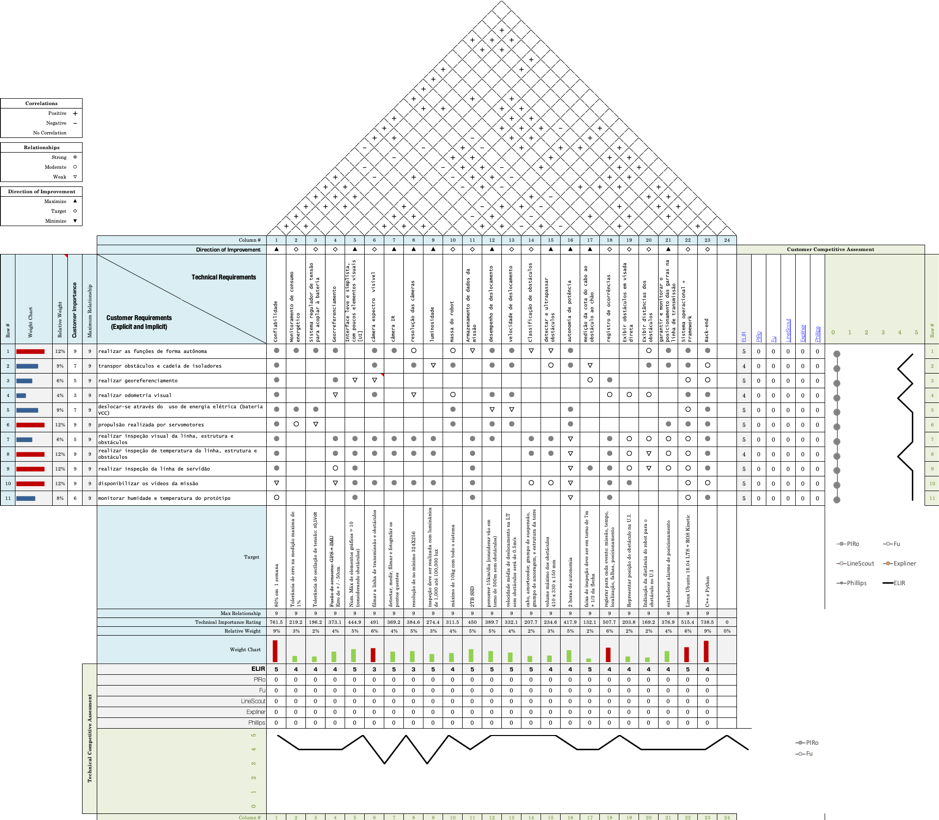
\includegraphics[scale=1]{Figures/qfdelir-2.png}
	\caption{QFD 2}
	\label{fig:qfd2}
\end{figure}

Com uma idealização do fluxo do sistema e suas funcionalidades, foi elaborada uma arquitetura geral do sistema de movimentação, mostrada na figura \ref{fig:arq_geral} e disponível no anexo X.  Antes do início da missão, é necessário que o sistema esteja apto a tal, assim foi definida uma funcionalidade para verificação da integridade do sistema, que requisita os status dos dispositivos antes de realizar a missão por meio de uma checagem, e com o sucesso na checagem, fornece o comando para o início.

\begin{figure}[H]
	\centering
	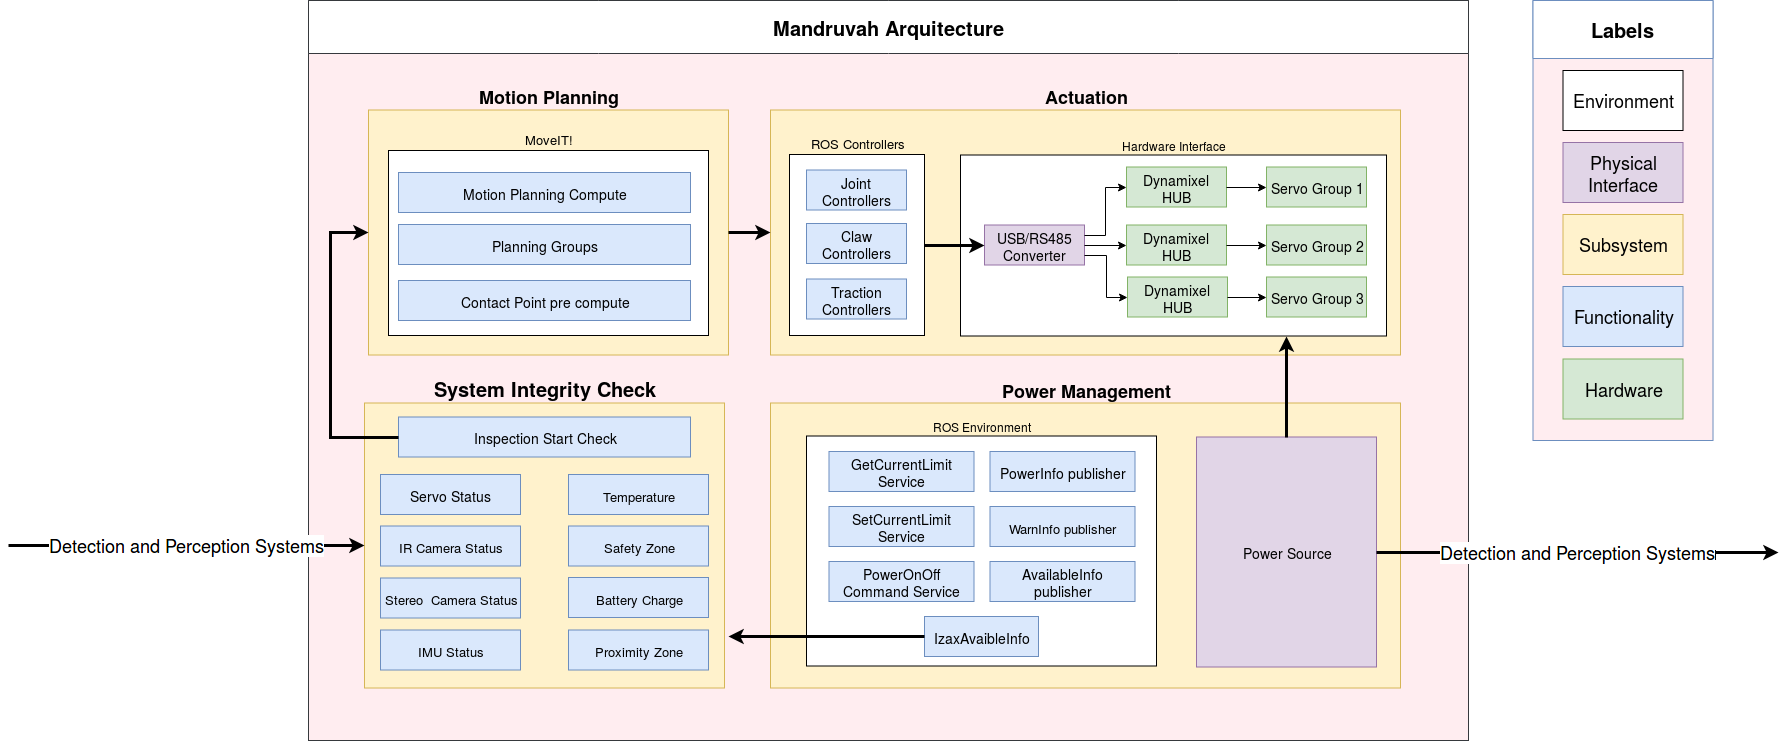
\includegraphics[scale=0.25]{Figures/Arquitetura.png}
	\caption{Arquitetura geral do sistema de movimentação}
	\label{fig:arq_geral}
\end{figure}
Determinou-se que a funcionalidade responsável pelo Planejamento de Movimento, realizasse o cálculo do plano de movimento junto com a administração dos grupos de controle e o cálculo de pontos de contato no robô. Onde essas informações sobre o plano de movimento do robô seriam transferidas para a funcionalidade de atuação do robô, que é responsável por receber esses comandos nas estruturas padrão do \textit{ROS} e realizar o movimento físico do robô.

A movimentação exige muita energia do robô e aliado à necessidade do controle da potência disponível, foi idealizada a funcionalidade de Gerenciamento de energia, responsável por disponibilizar as informações de energia no ambiente \textit{ROS} e fornecer a energia para o sistema de alimentação.

\subsection{Atuação}\label{sec:actuation}
Com a arquitetura geral do sistema de movimentação e o fluxo de comunicação, foi possível estabelecer as propriedades específicas da funcionalidade de atuação, onde buscou-se definir suas dependências, saídas e seu funcionamento.

Foi feito um fluxograma para representar a funcionalidade, onde estão ilustrados todos seus parâmetros, como mostra a figura \ref{fig:flux_atu}.

\begin{figure}[H]
	\centering
	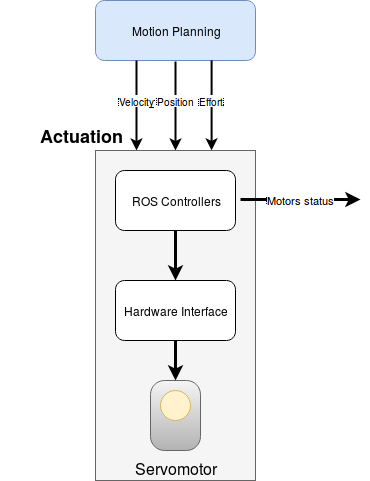
\includegraphics[scale=0.5]{Figures/actuation_depen.png}
	\caption{Fluxograma da funcionalidade de Atuação}
	\label{fig:flux_atu}
\end{figure}

Os comandos relativos a posição, esforço e velocidade para as juntas vêm da funcionalidade de planejamento de movimento, onde a atuação recebe esses comandos, transferindo os mesmos para os controladores do ambiente \textit{ROS} que se comunicam com a interface de \textit{hardware} que envia o comando para os motores realizarem o movimento.
\subsection{Planejamento de Movimento}\label{sec:plan_mov}
A forma que o robô vai realizar seus movimentos é determinado pela funcionalidade de Planejamento de Movimento. Que por sua vez tem a ferramenta \textit{MoveIt!} como importante componente para que a movimentação ocorra de forma efetiva, sendo assim, as unidades de \textit{software} da ferramenta que irão se comunicar com a funcionalidade explicitadas no fluxograma \ref{fig:fluxo_motion} estão incluídas no ambiente do \textit{MoveIt!}, recebendo o comando da posição desejada para o \textit{end-effector} e enviando os comandos necessários para as juntas. 
	
\begin{figure}[H]
	\centering
	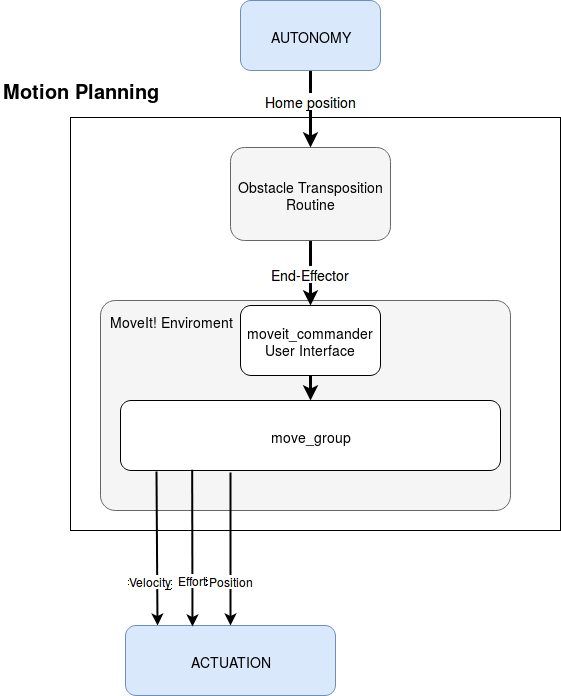
\includegraphics[scale=0.4]{Figures/motion_plan_func.png}
	\caption{Fluxograma da funcionalidade de Planejamento de Movimento}
	\label{fig:fluxo_motion}
\end{figure}

		
Apresenta uma dependência do sistema de autonomia do robô, que envia uma posição de referência o robô, o que culmina na necessidade da ultrapassagem de um obstáculo, já que, em operação, a ultrapassagem de obstáculos acontece diversas vezes. A rotina de ultrapassagem de obstáculo então envia para o \textit{software} o \textit{end-effector} necessário para a ultrapassagem, e consequentemente são enviados os comandos contendo  a posição, esforço e velocidades das juntas para a funcionalidade de atuação.

\subsection{Gerenciamento de Energia}\label{sec:geren_ener} 
A necessidade de distribuir a energia elétrica proveniente de uma bateria entre os sistemas eletrônicos do robô, de maneira inteligente se mostrou uma parte fundamental do projeto. Para que isso fosse implementado, houve a necessidade de desenvolver uma funcionalidade responsável por monitorar os níveis de corrente e tensão fornecidos para cada um dos dispositivos eletrônicos do robô, permitindo a criação de um sistema de proteção contra surtos de corrente, com ajuste de limites para valores do fornecimento de corrente.

Após a análise e constatação da necessidade da implementação desta funcionalidade, foram feitas as definições de quais seriam suas entradas, saídas e suas dependências.

A funcionalidade de gerenciamento de energia depende essencialmente da placa multiplexadora, a qual é responsável por alimentar o \textit{hardware} de \textit{Power Management} com a energia proveniente das baterias, e de que todos os seus drivers e funções estejam instaladas no ambiente \textit{ROS}, para que seja possível utilizar as suas ferramentas.

O sistema de \textit{power management} cria no ambiente \textit{ROS}, estruturas de \textit{software} responsáveis por permitir o monitoramento das portas de alimentação (informando valores de tensão e corrente), bem como a configuração dos limites do fornecimento de corrente e a desativação ou acionamento dos relés digitais de cada uma das portas.

O gerenciamento de energia monitora os valores de corrente fornecidos nas portas, e verifica  ocorrência de possíveis surtos, verificando o valor do pico e o tempo de duração. Caso seja detectado um surto de corrente, o fornecimento da porta é desativado, protegendo assim o sistema como um todo.

Uma vez que o estudo do \textit{hardware} e das suas funções no ambientes \textit{ROS} estavam completos, foram iniciados os primeiros testes com partes isoladas do robô para verificar o comportamento do \textit{hardware} e se o seu funcionamento estava de acordo com o esperado, para atender os requisitos da funcionalidade de maneira satisfatória, para assim ser integrado ao sistema.


\subsection{Checagem da Integridade do Sistema}\label{sec:check_sis}
Todas os sistemas do robô devem operar de maneira correta, para garantir o sucesso na execução da missão, e a partir desta observação, foi concebida a funcionalidade de checagem de integridade do sistema. Sua principal função é garantir que todas os sistemas do robô estejam sem apresentar falhas antes do início da missão. Uma vez que a checagem é realizada, o robô pode iniciar a sua missão.

Esta funcionalidade se mostra importante pelo fato de que a checagem prévia, reduz significantemente os riscos e prejuízos atrelados a uma má execução da missão, como componentes danificados e perda na eficiência durante toda a missão. Todos os sistemas que irão participar da missão, devem estar atrelados ao sistema por meio do ambiente \textit{ROS}, onde cada um irá informar o seu estado para a funcionalidade. O fluxograma \ref{fig:fluxo_check} foi desenvolvido para ilustrar o funcionamento da rotina de checagem integridade do sistema.

\begin{figure}[H]
	\centering
	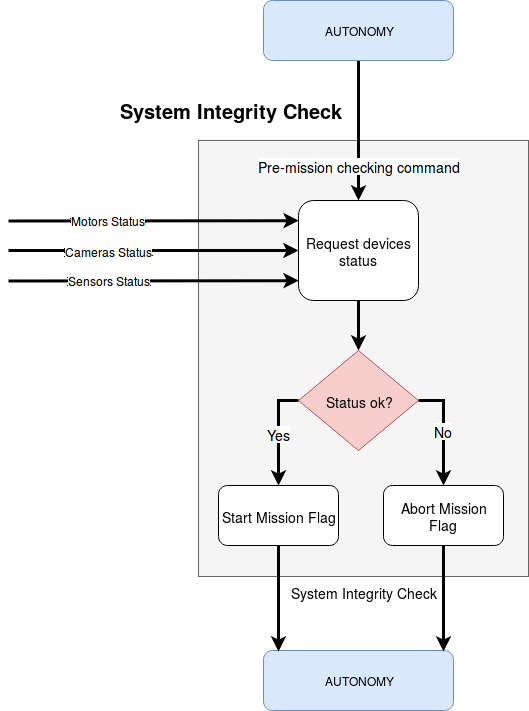
\includegraphics[scale=0.4]{Figures/sys_check_flux.png}
	\caption{Fluxograma da funcionalidade de Checagem da Integridade do Sistema}
	\label{fig:fluxo_check}
\end{figure}
Uma vez que esta funcionalidade foi concebida, toda as outras integrantes do sistema, deveriam se integrar ao sistema de integridade para garantir que a missão pudesse ser iniciada sem erros graves.

\section{Estudo da Movimentação}\label{sec:estud_mov}
Para o desenvolvimento das ferramentas para ultrapassagem de obstáculos, foi necessária a análise dos movimentos necessários para que fosse realizada a ultrapassagem de obstáculos. Os tipos de movimento a serem realizados influenciam nas ferramentas escolhidas para o controle e operação do robô, já que se busca a otimização do movimento e também redução do tempo gasto no desenvolvimento, de forma a garantir um resultado satisfatório.

Foi feita uma análise utilizando como referência o maior obstáculo, que foi o amortecedor, mostrado na figura \ref{fig:amortecedor} e levando em consideração a sua modelagem como um paralelepípedo de maior dimensão 535mm. Constatou-se que seria necessário que para a ultrapassagem desse obstáculo, o robô necessitaria abrir um dos braços e se deslocar somente com a unidade de tração central e outro braço. Para isso seriam necessários movimentos para abrir e fechar as garras do robô, assim como um comando específico para afastar a unidade de tração da linha a distância necessária para a abertura da garra. Assim como o movimento que abre o braço o suficiente para que esse passe abaixo do obstáculo.

\begin{figure}[H]
	\centering
	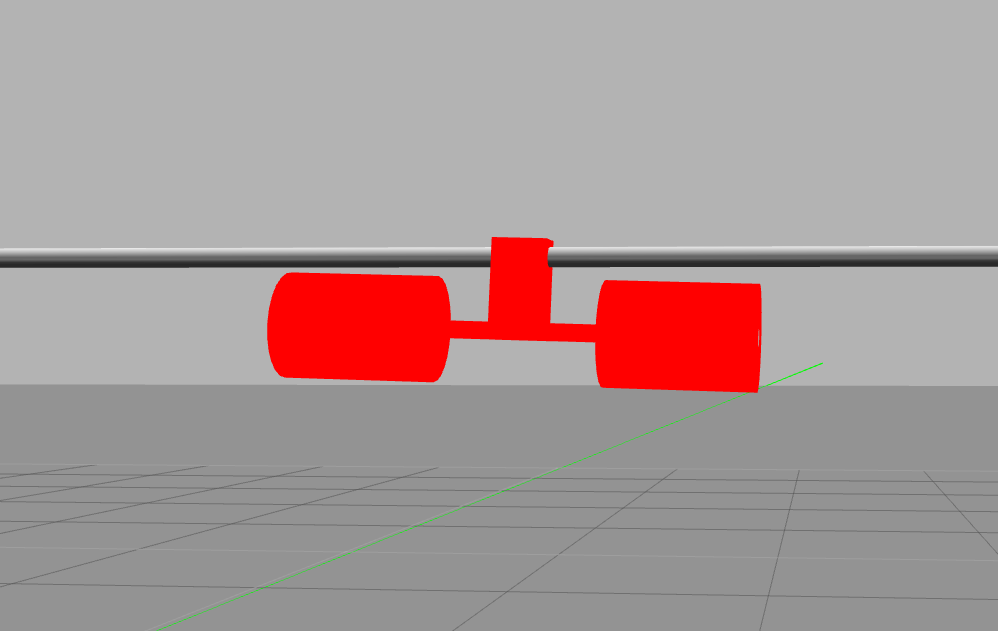
\includegraphics[scale=0.25]{Figures/obstaculo.png}
	\caption{Visualização do obstáculo no simulador}
	\label{fig:amortecedor}
\end{figure}

A ferramenta de visualização presente no \textit{ROS}, possibilitou testar os limites de giros das juntas e visualizar como seriam as poses do robô sem a necessidade da simulação. O conhecimento relacionado à como a movimentação ia ocorrer possibilitou nortear o desenvolvimento.

\begin{figure}[H]
	\centering
	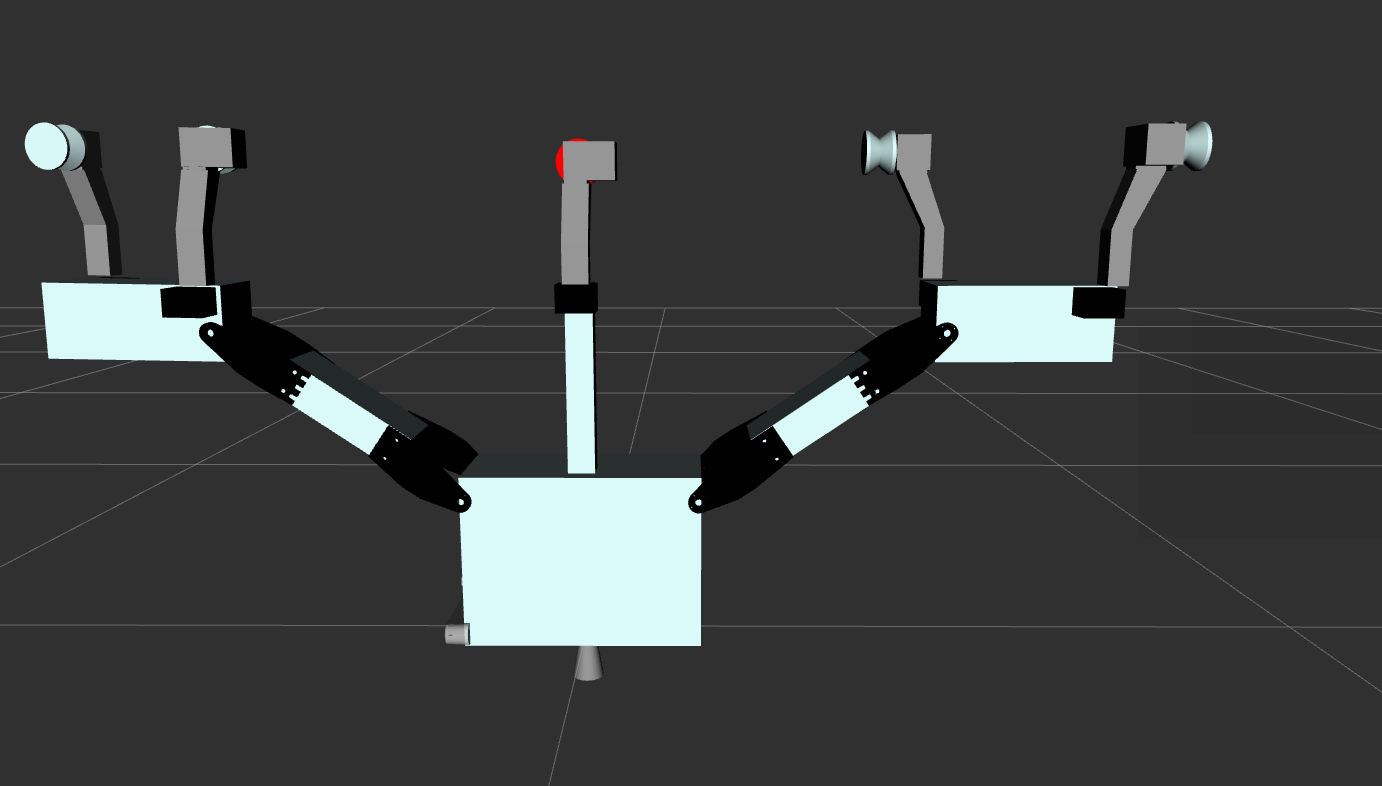
\includegraphics[scale=0.25]{Figures/rviz_garra_aberta.png}
	\caption{Robo \textit{ELIR} no visualizador do \textit{ROS} com garras abertas}
	\label{fig:elir_garras abertas}
\end{figure}
\section{Soluções Mecatrônicas para o sistema robótico}\label{sec:sol_sis}
Uma vez que os principais aspectos das funcionalidades estavam definidos, foi necessário realizar a implementação das soluções mecatrônicas no robô. Foram realizados estudos de dispositivos eletrônicos e das suas ferramentas de configuração, bem como programas e \textit{software}s que seriam necessários para a implementação das funcionalidades.

\subsection{Escolha a biblioteca de controladores no \textit{ROS}}\label{sec:contr_ros}
Para implementar as rotinas de controle e atuação dos motores Dynamixel, era necessário que houvesse algum meio de configurá-lo para operar de maneira desejada, podendo realizar a criação de juntas, e unidades de tração. Especificamente nos motores Dynamixel, isto é possível através da utilização de \textit{drivers}.

Os \textit{drivers} são estruturas de \textit{software} que permitem a compatibilização do dispositivo físico com uma interface computacional, habilitando as suas funções e configurações dentro de um ambiente de \textit{software}, permitindo que o dispositivo possa ser configurado e ter suas funções utilizada através de comandos provenientes de uma camada de \textit{software} superior.

A movimentação das juntas e eixos do robô se dá pelo uso de servomotores, e para que os mesmos sejam controlados pelo \textit{framework}, que no caso é o \textit{ROS} - é necessário fazer uso de um \textit{driver}.

Diante a variedade de bibliotecas para controlar os motores da dynamixel no \textit{ROS} disponíveis, foi necessário escolher qual será utilizada. Para escolha a biblioteca foram levados alguns parâmetros que influenciam para o fluxo de informações e funcionalidades do robô, assim como complexidade de código, disponibilidade de tutoriais, suporte pela comunidade, as ferramentas disponíveis, compatibilidade do \textit{firmware}, etc.

Foram selecionadas 2 bibliotecas que são disponibilizadas pelo próprio \textit{framework} \textit{ROS}, sendo elas: a  \textit{dynamixel\_drivers} e a \textit{dynamixel\_workbench}. A escolha pela \textit{dynamixel\_drivers} se deu pelo fato ser mais velha e por consequência mais materiais disponíveis para consulta, apesar a \textit{workbench} possuir suporte para novas versões do Dynamixel, essa possibilidade não teve muitos benefícios, já que o projeto foi utilizado para versões antigas de motores. 

\subsection{Solução para cinemática}\label{sec:sol_cine}
O cálculo da cinemática pode ser realizado de diferentes formas, já que o mesmo parte da modelagem do robô por meio de um conjunto de equações. Existem diferentes solucionadores para problemas de cinemática, que podem utilizar diferentes parâmetros de entrada.

No âmbito da robótica podem ser utilizados tanto os modelos matemáticos já elaborados pelos desenvolvedores, como também o modelo 3D do robô. Esse modelo 3D é definido geralmente por meio de arquivos do tipo \textit{URDF} , que utilizam uma escrita simples, definindo o robô a partir de seus \textit{links} e juntas. Esse arquivo é o mesmo utilizado para colocar o modelo do robô na simulação, e também é a forma padrão utilizada pelo \textit{software} \textit{MoveIt!}.
Com o estudo do estado da arte fornecido, não era necessário encontrar o conjunto de equações que descrevem o robô, e com a simulação fornecida, também já era possível utilizar o modelo \textit{URDF}. Foi feita uma análise entre as possíveis soluções cinemáticas, buscando encontrar a que garantisse um maior sucesso e facilitasse o desenvolvimento. Levando em consideração a disponibilidade de códigos e tutoriais para serem tomados como base, assim como o uso em projetos semelhantes, a complexidade da aplicação e integração com as estruturas do \textit{ROS}.

Assim levantou-se 3 possível soluções para o cálculo da cinemática inversa, sendo elas: o uso do modelo matemático já existente proveniente do estudo do estado da arte, sendo realizada sua solução manualmente por meio de códigos de programação, o uso da ferramenta \textit{MoveIt!} utilizando o modelo \textit{URDF} proveniente da simulação, e o uso da ferramenta \textit{MoveIt!} compatibilizada com modelo matemático.

A uso do modelo matemático completo para o robô, realizando a  solução por meio de um código, se mostrou inviável, já que também seria necessário a integração com as estruturas de controle do \textit{ROS}, e mesmo a implementação desse modelo no \textit{MoveIt!} não se mostrou a melhor opção, devido a alta complexidade e a falta de projetos semelhantes para consulta, tal qual a inexistência de tutoriais voltadas para essa aplicação em específico. Assim sendo escolhido o uso da ferramenta \textit{MoveIt!} com o modelo \textit{URDF} proveniente da simulação, já que esse mesmo modelo já é estudado pela equipe, para seu uso na simulação e a aplicação padrão do \textit{MoveIt!} utiliza esse modelo.

Essa solução utiliza os dados sobre o modelo do robô contidos no modelo \textit{URDF} para realizar o cálculo da cinemática de forma analítica, gerando diversas trajetórias e encontrando a melhor possível, baseada nos parâmetros configurados pelo usuário.

\subsection{Gerenciamento de Energia}\label{sec:geren_ene}
A implementação da funcionalidade de gerenciamento de energia foi possível através da utilização de um \textit{hardware} de \textit{Power Management}, uma placa eletrônica, fornecida pelo cliente do projeto, iniciando assim a primeira etapa do desenvolvimento da funcionalidade de gerenciamento de energia, a qual se deu pelo estudo do \textit{hardware}, através da leitura de \textit{datasheets} e esquemas elétricos. 

A placa contém sete portas de alimentação gerenciadas por relés digitais sendo cinco delas de 12 Volts e duas de 5 Volts. Dentre as portas de 12 Volts, 4 possuem regulação de fornecimento de corrente, onde o controle do fornecimento é realizado por um microcontrolador Atmega32U4. Todas as portas possuem sensores de tensão e corrente individuais, facilitando e otimizando o processo de leitura dos . O \textit{firmware} embarcado na placa de \textit{Power Management} possui a principal de função de implementar os relés digitais, onde se realiza uma leitura dos valores de corrente que estão sendo demandados pelas portas. 

Para que a integração do \textit{hardware} de \textit{Power Management} fosse realizada ao projeto foi necessário validar o seu funcionamento , e se os valores de tensão fornecidos, estariam de acordo com o configurado. As medições lidas no multímetro e no \textit{software}, foram registradas e comparadas, verificando se os valores de erro eram muito altos. Como mostra a Tabela \ref{tab:med_pow} a seguir:

\begin{table}[H]
	\centering
	\caption{Medições de tensão para o \textit{hardware} de \textit{Power Management}}
	\label{tab:med_pow}
	\begin{tabular}{ccc}	
		\hline
		\multicolumn{1}{r}{Porta Lida}      & Tensão - Multímetro         & Tensão - \textit{Software}         \\ \hline
		Porta 1                                            & 12.03 Volts          & 12.043 Volts     \\ \hline
		Porta 2                                           & 12.01 Volts     & 12.037 Volts          \\ \hline
		Porta 3                                           & 12.01 Volts     & 12.038 Volts          \\ \hline
		Porta 4                                           & 12.01 Volts     & 12.037 Volts          \\ \hline
	\end{tabular}
\end{table}
Foi possível perceber uma pequena variação na leitura em \textit{software} para a leitura realizada pelo instrumento de medição, apesar disso, pelo fato do erro ser de uma ordem baixa para os níveis de operação do robô, considerou-se que esta variação não representaria risco para a operação, validando assim o funcionamento do \textit{hardware} da \textit{Power Management}.


\section{Simulação}\label{sec:simul_result}
A estrutura do sistema \textit{ROS} e suas ferramentas já compatibilizada faz com que a simulação do sistema impacte de forma efetiva e positiva durante o processo de desenvolvimento. O \textit{software} Gazebo é uma das ferramentas para simulação  de ambientes robóticos mais utilizadas atualmente, por apresentar integração nativa com o sistema \textit{ROS} e foi utilizada para o projeto.

Os arquivos para  simulação do robô foram fornecidos pelo cliente, e apresentam características semelhantes às esperadas no robô real, como o tipo dos controladores de juntas, que são o padrão do \textit{ROS}, sendo os mesmos utilizados para o robô real, e consistindo assim um parâmetro fundamental para a simulação do sistema de movimentação.

Por apresentar os mesmos tipos de controladores do robô real, foi possível utilizar a simulação para validar a compatibilização do controle da ferramenta \textit{MoveIt!} com os controladores presentes no robô. Essa alternativa possibilitou a compatibilização entre as funcionalidades sem a necessidade do protótipo do robô pronto funcional, economizando tempo do desenvolvimento, já que reduz dependência entre as fases do desenvolvimento.

\subsection{Simulação para a rotina de ultrapassagem}\label{sec:simu_ultr}
A automatização dos movimentos do sistema é necessária para que ocorra a ultrapassagem, sendo assim esse conjunto de movimentos denominado de rotina. As estruturas do \textit{ROS} possibilitam a criação de estruturas que quando acionadas realizam comandos específicos.

Por apresentar os mesmo controladores, e com o auxílio do estudo dos movimentos necessários para a ultrapassagem, foi possível desenvolver os códigos que enviam os comandos específicos para os controladores. 

Com uso da simulação foi possivel desenvolver e testar os serviços do ROS, na figura \ref{fig:simu_garras_abertas} é possível observar o serviço de suspender o conjunto de garras em funcionamento:

\begin{figure}[H]
	\centering
	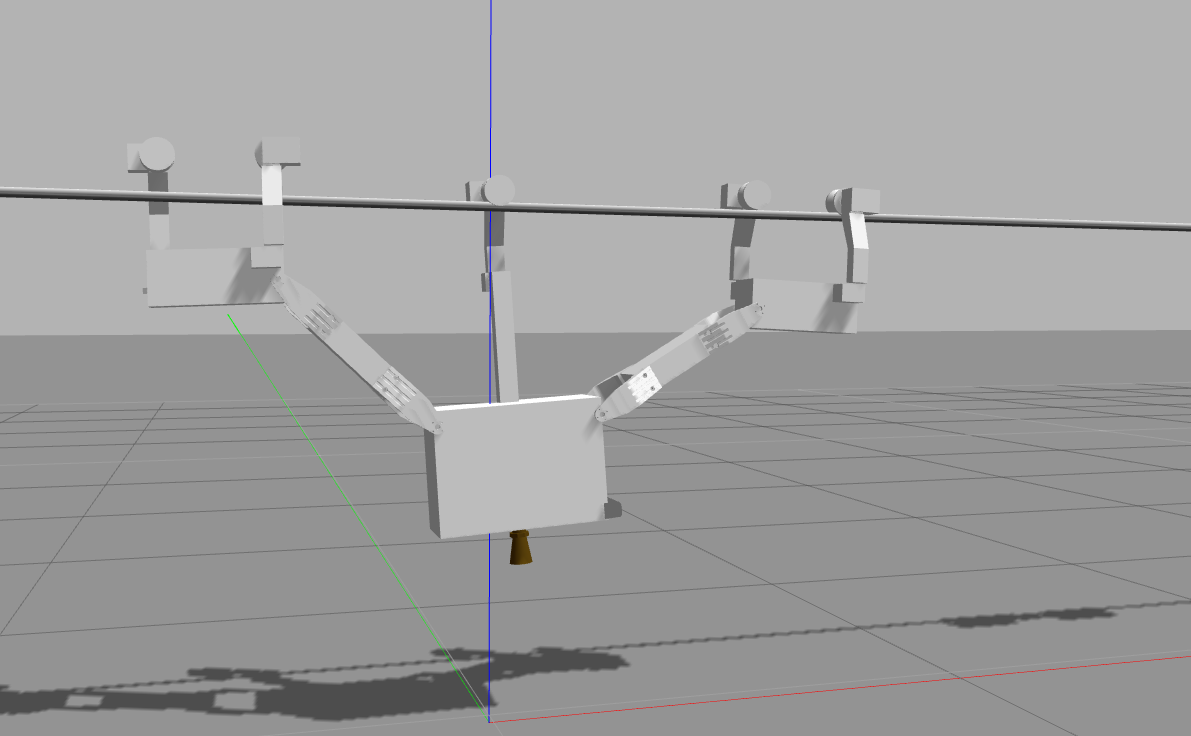
\includegraphics[scale=0.25]{Figures/servico_simulacao_subirgarra.png}
	\caption{Robo \textit{ELIR} no \textit{Gazebo} com garras abertas}
	\label{fig:simu_garras_abertas}
\end{figure}

\section{Testes de Movimentação Física}\label{sec:test_mov}
Os testes de movimentação física buscam compreender e validar os movimentos realizados pelo robô, indo desde da análise individual das partes do robô como braços e unidade de tração, até sua movimentação em conjunto.

\subsection{Testes unitários}\label{sec:test_mov_uni}
Os primeiros testes foram feitos com a estrutura parcialmente montada, já que o objetivo do teste é validar o funcionamento dos controladores de junta do \textit{ROS}, que é a base para o desenvolvimento das funcionalidades de Atuação e Planejamento da Movimentação. Nestes testes, foram estabelecidos os limites de movimentação das juntas, com o intuito de preservar a integridade física dos componentes. As juntas dos braços do robô \textit{ELIR} são compostas por dois servomotores Dynamixel MX-106R fabricados pela Robotis. 

No decorrer desses primeiros testes, ocorreram falhas nos motores por excesso de carga em um deles, o que era configurado como mestre. Verificou-se que isso poderia ser contornado com o uso do cabo de sincronização ligando os dois motores de cada junta, já que os motores se comunicariam diretamente entre si para balancear a divisão da carga sobre a junta. Também foi o momento de analisar como se comportavam os servomotores utilizados nas juntas, sob influência do cabo de sincronização.
\begin{table}[H]
	\centering
	\caption{Sentido de giro dos motores (Cabo de sincronização direto)}
	\begin{tabular}{ccc}	
			\hline
		\multicolumn{1}{r}{Valor pulicado na junta:}      & Positivo         & Negativo         \\ \hline
		Mestre                                            & Horário          & Anti-horário     \\ \hline
		Escravo                                           & Anti-horário     & Horário          \\ \hline
	\end{tabular}
\end{table}

\begin{table}[H]
	\centering
	\caption{Sentido de giro dos motores (Cabo de sincronização cruzado)}
	\begin{tabular}{ccc}
		\hline
		
		\multicolumn{1}{r}{Valor pulicado na junta:}       & Positivo       & Negativo           \\ \hline
		Mestre                                             & Horário        & Anti-horário       \\ \hline
		Escravo                                            & Horário        & Anti-horário       \\ \hline
	\end{tabular}
\end{table}

Levando em conta que, para realizar o movimento corretamente, os motores tem que se movimentar em sentidos opostos, já que estão fisicamente invertidos, caso seja utilizado o cabo de sincronização cruzado, os motores escravos devem ser configurados com o modo de giro reverso.

\subsection{Testes na linha de transmissão}\label{sec:test_mov_lin}
O teste no ambiente onde o robô irá operar é de suma importância para o seu desenvolvimento. Tendo como finalidade verificar o comportamento do robô e seus sistemas  nessa situação, foram realizados testes de movimentação na linha de transmissão buscando executar etapas que fazem parte da rotina de ultrapassagem. Para verificar o deslocamento horizontal por meio de roldanas, realizou-se um testes posicionando robô na linha e controlando somente as unidades de tração das roldanas, verificando assim que elas poderiam se soltar da linha. Dessa maneira, concluiu-se que as garras onde estão as roldanas deveriam ter o seu torque habilitado para travá-la na posição, para que o robô não se desprenda da linha.

Durante os testes de movimentação na linha, foram testadas outras etapas da rotina de ultrapassagem. Quando o braço era levantado para retirar as roldanas da linha, todo o robô se inclinava para a frente.  Levantou-se a hipótese de que, o fato das juntas dos braços estarem "relaxadas" permitia essa inclinação. O teste foi repetido com o torque destas juntas habilitado, dessa forma o problema foi contornado.



\section{Integração com os subsistemas}\label{sec:int_subsis}
Após a validação do funcionamento dos subsistemas, verificando se estão operando corretamente através dos testes unitários, foi necessário conferir o funcionamento do sistema como um todo, analisando a integração das as funcionalidades, com o objetivo de observar se houveram erros no processo de integração. Os testes buscavam seguir com integração simples entre funcionalidades, até os testes finais, envolvendo todas as funcionalidades desenvolvidas durante o projeto.

\subsection{Teste dos servomotores em rede}\label{sec:test_serv_red}
Como o robô \textit{ELIR} possui ao total 18 servomotores Dynamixel, então torna-se  importante verificar o seu comportamento quando todos estão pertencendo a mesma malha de controle. Para isso foi utilizado \textit{hubs} para a separação em 3 grupos, contendo 6 motores por grupo. Para efetuar o teste foi utilizado a biblioteca dos controladores do \textit{ROS} que indica quantos motores estão conectados a unidade de processamento.

Cada grupo de motor foi testado separadamente e todos os 3 foram encontrados, concluindo que as ligações, alimentação e comunicação foram feitas corretamente. Mas ao colocar os 3 grupos de motores, percebeu-se que nem todos os motores eram encontrados.

Buscou-se reduzir as fontes de erro, realizando uma verificação na alimentação e nas ligações responsáveis pela comunicação entre os motores, o que não foi eficiente, assim como a restauração do \textit{firmware} de cada um. Como não haviam mais fontes de erro, buscou-se encontrar motores que poderiam estar induzindo esse problema no sistema. Assim, foi pensado em adicionar motor por motor para observar o comportamento e a partir disso analisou-se que somente 2 motores específicos causavam falhas na rede, constando que os mesmo estavam com problemas em comunicação em rede e que vieram com defeitos de fábrica. Logo após a troca dos motores defeituosos a comunicação ocorreu de forma coerente e constatou-se que os 18 motores conseguem se comunicar em redes grandes.

\subsection{Teste de movimentação alimentada por banco de baterias}\label{sec:test_bate}
Para que o robô \textit{ELIR} desempenhasse suas funções de forma autônoma era necessário o uso de baterias que suportasse toda demanda energia do mesmo. Afim de saber quantas baterias iriam ser usadas dentro da estrutura do robô, foi feito uma estimativa a partir 

Durante todo desenvolvimento do projeto foi utilizado fontes de bancada onde a tensão era de 14V onde os motores desempenham maior torque 
Antes de utilizar as baterias para que o robô pudesse realizar os movimentos na linha, tornou-se importante realizar testes para garantir que a mesma, juntamente com a placa de gerenciamento de energia, fornecem potência suficiente com tensão a 12V para que os motores realizem sua movimentação.
Com isso, era interessante verificar por quanto tempo os motores aguentariam na posição que demanda maior torque no qual possui maior carga devido ao momento aplicado ao braço, como mostrada na figura \ref{fig:robo_pior_pos} a seguir:
\begin{figure}[H]
	\centering
	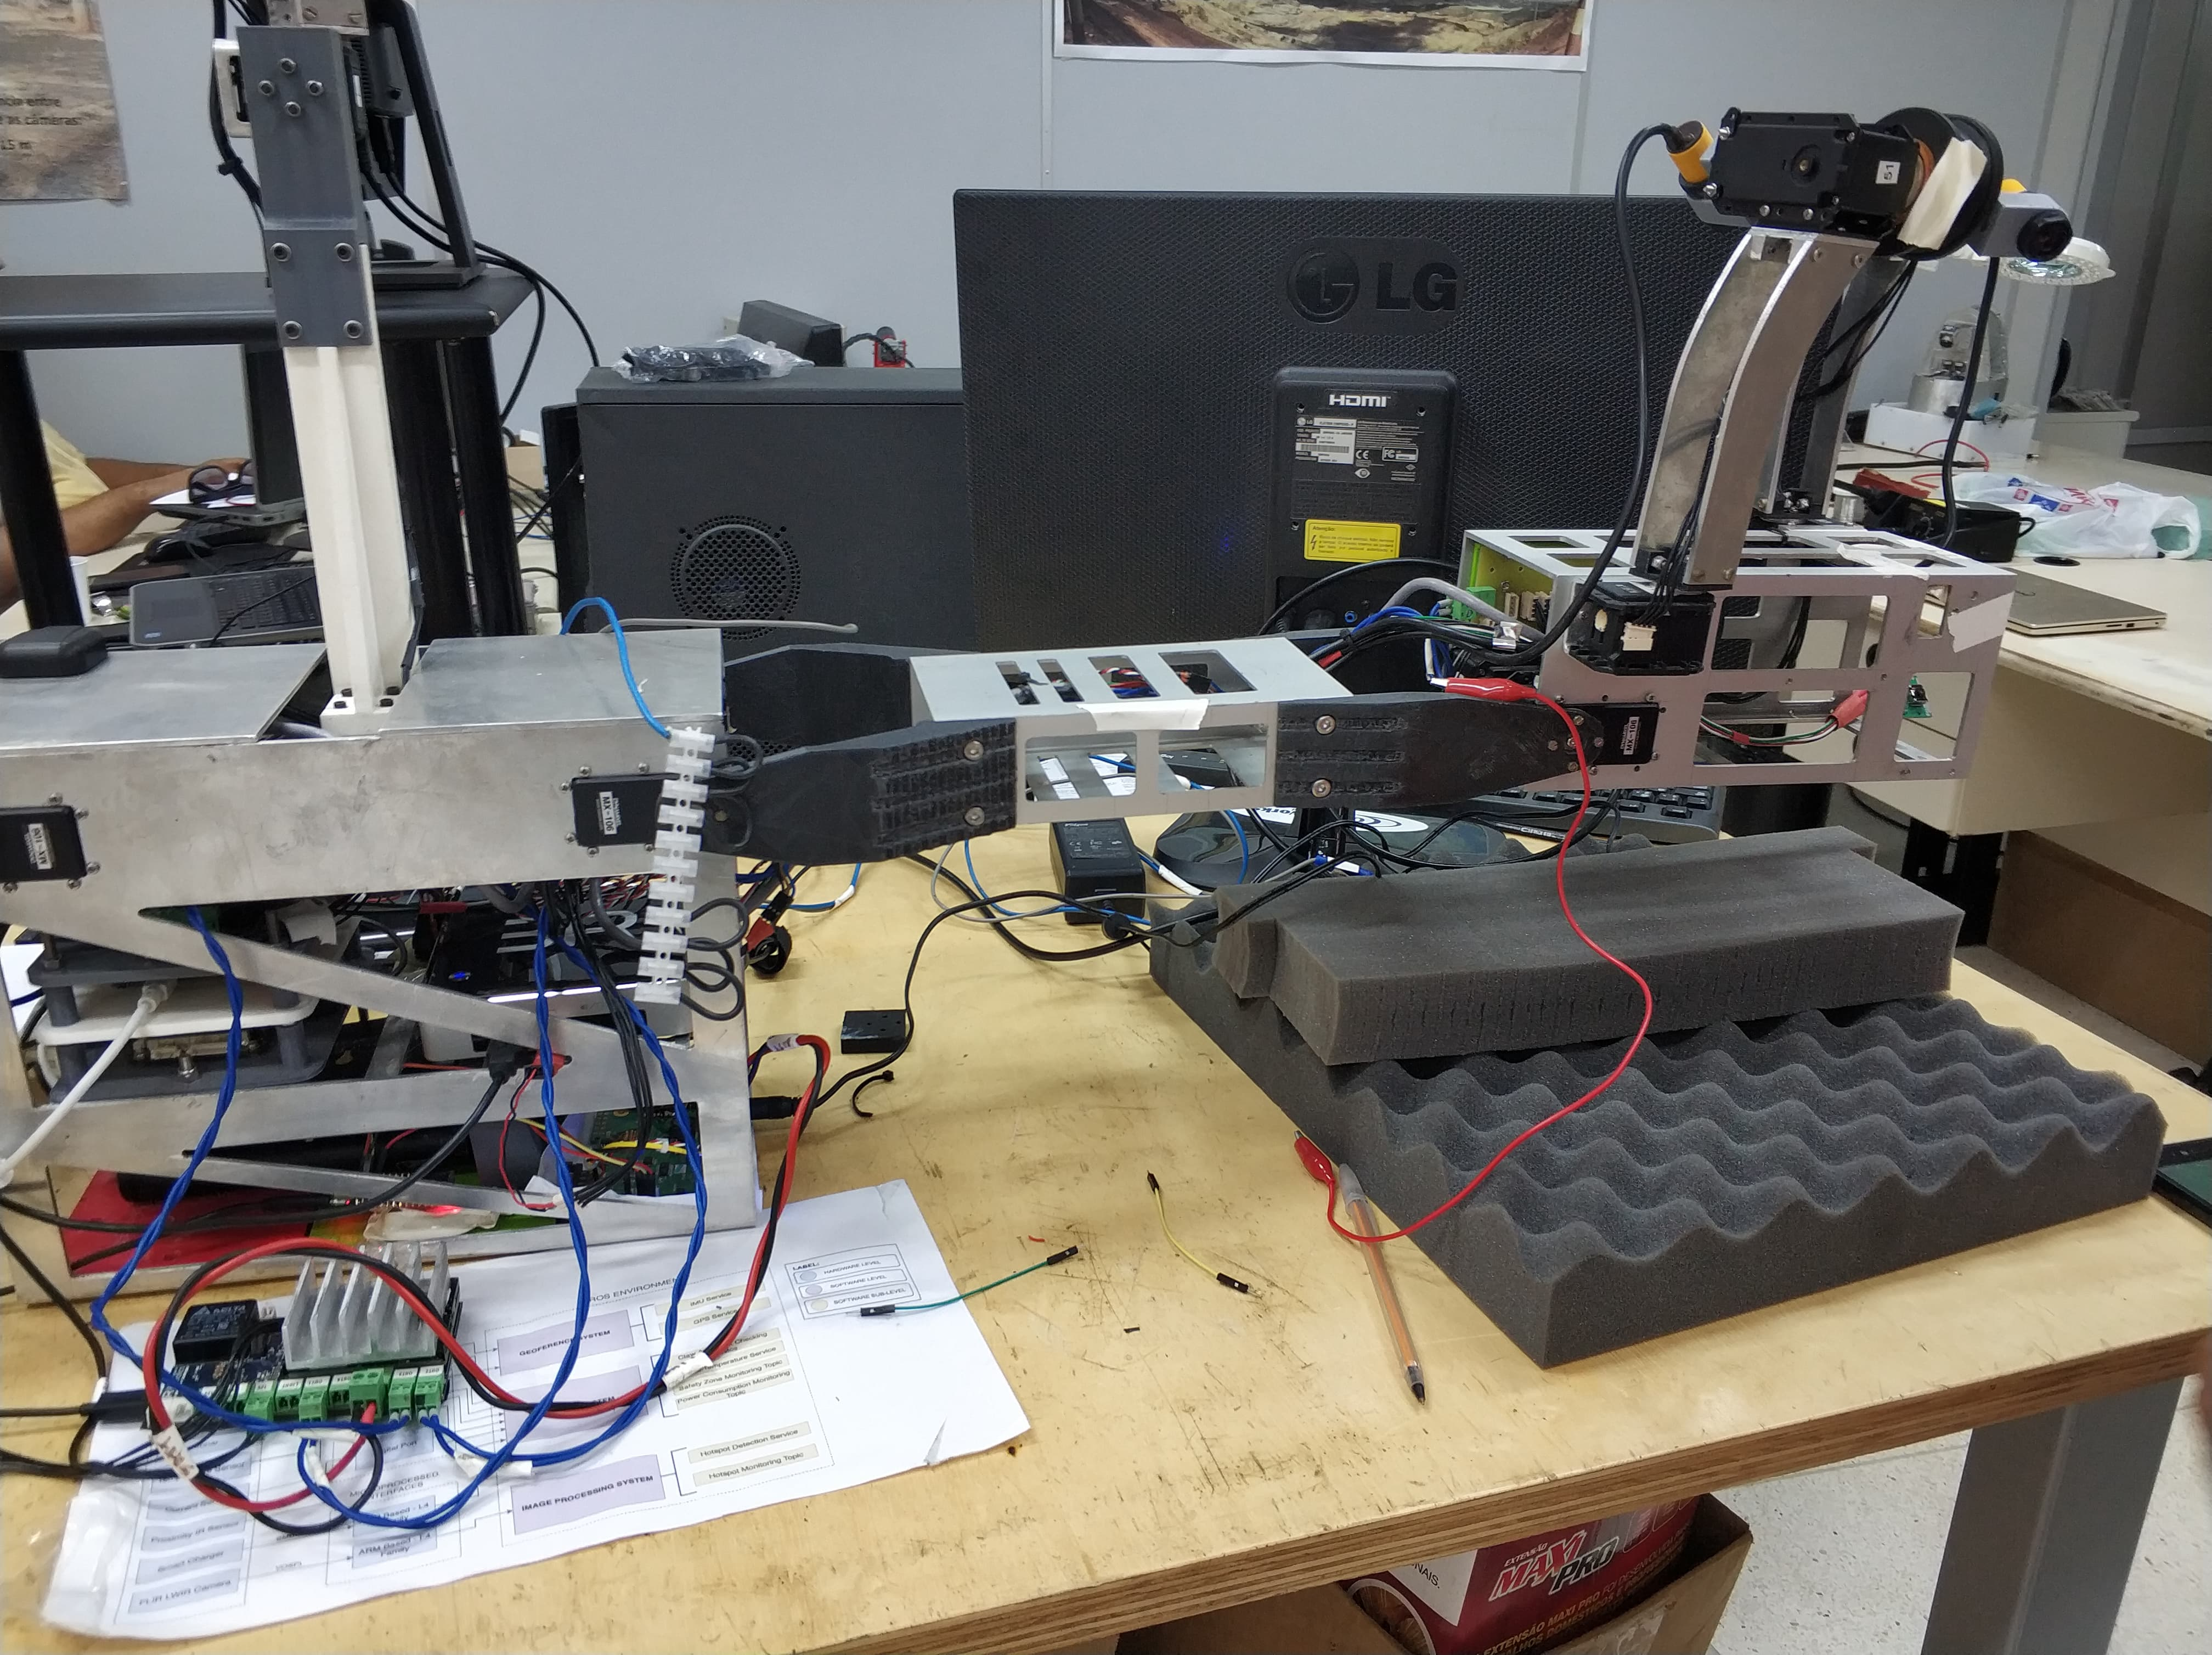
\includegraphics[scale=0.08]{Figures/robo_pior_posicao.jpg}
	\caption{Foto do robô na posição que demanda maior torque}
	\label{fig:robo_pior_pos}
\end{figure}

Verificou-se que o robô respondeu bem com as baterias ficando nesta posição durante 10 minutos por 3 vezes, validando o seu uso e comprovando que os motores a 12V fornecidos pela placa realizam torque suficiente para a carga da estrutura.

\section{Análise Preliminar}\label{sec:anal_prem}

Algumas situações só são expostas durante o desenvolvimento do projeto, com a aplicação das ferramentas e a vivência de testes. O desenvolvimento do projeto passou por diversas etapas, onde fora necessário realizar o retrabalho de novos estudos sobre as problema de compatibilização do modelo do robô dentro da plataforma \textit{MoveIt!}, uma vez que o \textit{software} não funciona bem com robôs que possuem apenas dois graus de liberdade, o que é o caso do robô \textit{ELIR}. A observação desse erro é fundamental para o processo de aprendizado no que tange ao desenvolvimento de robótica, tornando o \textit{MoveIt!} uma solução não indicada para o problema da solução da cinemática inversa, porém ainda se mostra muito útil para o planejamento do movimento e integração com outras tecnologias, assim compensando a solução da cinemática manualmente, para projetos de menor complexidade.

Em termos de hardware, os erros que surgiram também foram importantes para ilustrar melhor como os mesmos deveriam ser configurados de maneira correta e também as suas limitações de trabalho, a exemplo dos motores \textit{Dynamixel}, estes mostraram um desempenho mais efetivo ao trabalhar com tensões mais elevadas, 14V ao invés dos tradicionais 12V, diminuindo a corrente demandada durante a operação, otimizando o consumo.      

Ainda se tratando do uso dos motores, a necessidade do uso dos cabos de sincronização para evitar erros de sobrecarga foi um fator crucial para o desenvolvimento do projeto. Neste ponto observou-se que os motores, ao trabalharem como \textit{dual}-\textit{joint} (junta com dois motores), necessitam do uso de cabos de sincronização para transmitir a informação de carga necessária para realização do movimento, balanceando o esforço realizado pelos motores trabalhando em conjunto.


